\chapter{Pre-study} 

\section{Academia}

Within the academic community, 
there exists a concerted effort to address issues related to energy efficiency and the adoption of renewable energy sources. 
There are numerous research and ongoing projects aimed at establishing a robust social energy infrastructure capable of adapting to the utilization of renewable energy sources. 
Studies are also investigating the feasibility and practicalities of establishing zero-emission households and buildings.
Technological innovations designed to support these goals have also been a focal point in the academic discourse surrounding energy efficiency and the transition to renewable energy.

In the meantime, Palmer et al. \cite{informationgap} drew attention to the fact that engineering studies have identified various investments in new energy-efficient equipment or building retrofits that would generate savings surpassing their costs in terms of lower future energy expenses. However, homeowners and businesses lack sufficient knowledge and guidance on how to effectively utilize these opportunities to their advantage.

\section{Industry}


\section{Regulations}


%Empirical results suggest that households' propensity to invest in clean energy technologies depends mainly on home ownership, income, social context and household energy conservation practices,
%in addition, environmental attitudes and beliefs, as manifest in energy conservation practices or membership in an environmental non-governmental organisation, also play a relevant role in technology adoption \cite{determinants}.


\section{The newTRENDs project}

Renewable energy (\gls{re}) and energy efficiency (\gls{ee}) are two central strategies pursued by the \gls{eu} and its Member States concerning the energy system. 
%In 2019, 80.9\% of our total energy supply still depended on burning fossil fuels, namely 26.8\% coal, 30.9\% oil and 23.2\% natural gas \cite{iea}. 
Investments into low-carbon power generation accounted for 15\% recently are expected to rise to more than 30\% by 2030, corresponding to a quadrupling in absolute volumes \cite{shift}. Solar, wind, and the investments for enabling the integration of these technologies to the grid dominate the investments into low-carbon power generation \cite{shift}. 
%Electrification is playing a major role in the energy transition process. 
%Meanwhile, different electrification strategies rely heavily on energy efficiency \cite{electrification}.
Measures to increase energy efficiency, including investments in energy savings and the consolidation of consultancy and information services, are promoted by The National Action Plan on Energy Efficiency (\gls{nape}) \cite{bafa}.  

Transitioning towards a sustainable energy system necessitates significant effort on both the demand and supply sides. 
However, previous research has shown that in many areas energy efficiency gains were counteracted by societal trends that increased corresponding activities, leading to much smaller decreases (or even increases) of energy demand than technologically feasible \cite{2050}. 
The aim of newTRENDs is to increase the qualitative and quantitative understanding of impacts of new societal trends on energy consumption and to improve the modelling of energy demand, energy efficiency and policy instruments \cite{fraunhofer}. 


%%%%%%%%%%%%%%%%%%%%
\subsection{New societal trends on energy demand}


Researchers believe new societal trends have the potential to shift energy demands between sectors and might reinforce or diminish one another when they occur at the same time \cite{2050}. 
%Researchers and organisations are paying increasing attention to how new societal trends are affecting energy demand.
It is therefore important to access current and (foreseeable) future societal trends concerning the impact that they might have on future energy demand \cite{2050}. 

Four arising societal trend clusters that are likely to shape future energy demand in European countries (and worldwide) were established by Brugger et al. \cite{2050}:  
\emph{
  (1) the digitalization of the economy and of private life; 
  (2) new social and economic models, including the sharing economy and prosumaging (combination of producing, consuming and managing of energy); 
  (3) industrial transformation, including decarbonization of industrial processes and the circular economy (including a stronger focus on material efficiency); 
  (4) quality of life, including health effects, urbanization and regionalization. 
}

%\begin{itemize}
%  \item \textbf{Digitalization of life} %\\ the digitalization of the economy and of private life;
%  \item \textbf{New social and economic models} %\\ including the sharing economy and prosumaging (combination of producing, consuming and managing of energy);
%  \item \textbf{Industrial transformation} %\\ including decarbonization of industrial processes and the circular economy (including a stronger focus on material efficiency);
%  \item \textbf{Quality of life} %\\ including health effects, urbanization and regionalization. 
%\end{itemize}

%The newTRENDs project develops the analytical basis for a “2050 Energy Efficiency Vision” by considering new societal trends in energy demand modeling \cite{newtrends}. 
Considering the impact of these new societal trends on energy demand from a closer sectoral perspective,
Yu et al. \cite{newtrends} identified four energy sectors: 

\begin{itemize}
  \item industry, 
  \item transport,  
  \item tertiary, 
  \item residential.  
\end{itemize}

This proposed thesis will focus on the residential sector 
while taking scenarios of “consumers” becoming “prosumers” (with \gls{pv}) and “prosumagers” (adding energy storage and \gls{sems}) \cite{consumer} into account.  


%%%%%%%%%%%%%%%%%%%%
\subsection{The modeling of residential buildings}


The FLEX models of the newTRENDs project are referred to as “RC models”,
that calculate (simulate or optimize) the building energy demand at the hourly resolution,
considering the trends of prosumaging households and energy communities, 
which significantly supports the analysis of relevant policies promoting the diffusion of heat pumps (\gls{hp}), \gls{pv}, batteries, and \gls{sems} \cite{newtrends}.


The figure \ref{fig:flex} shows how FLEX interacts with other bottom-up models involved in the newTRENDs project.

\begin{figure}[h]
  \centering
  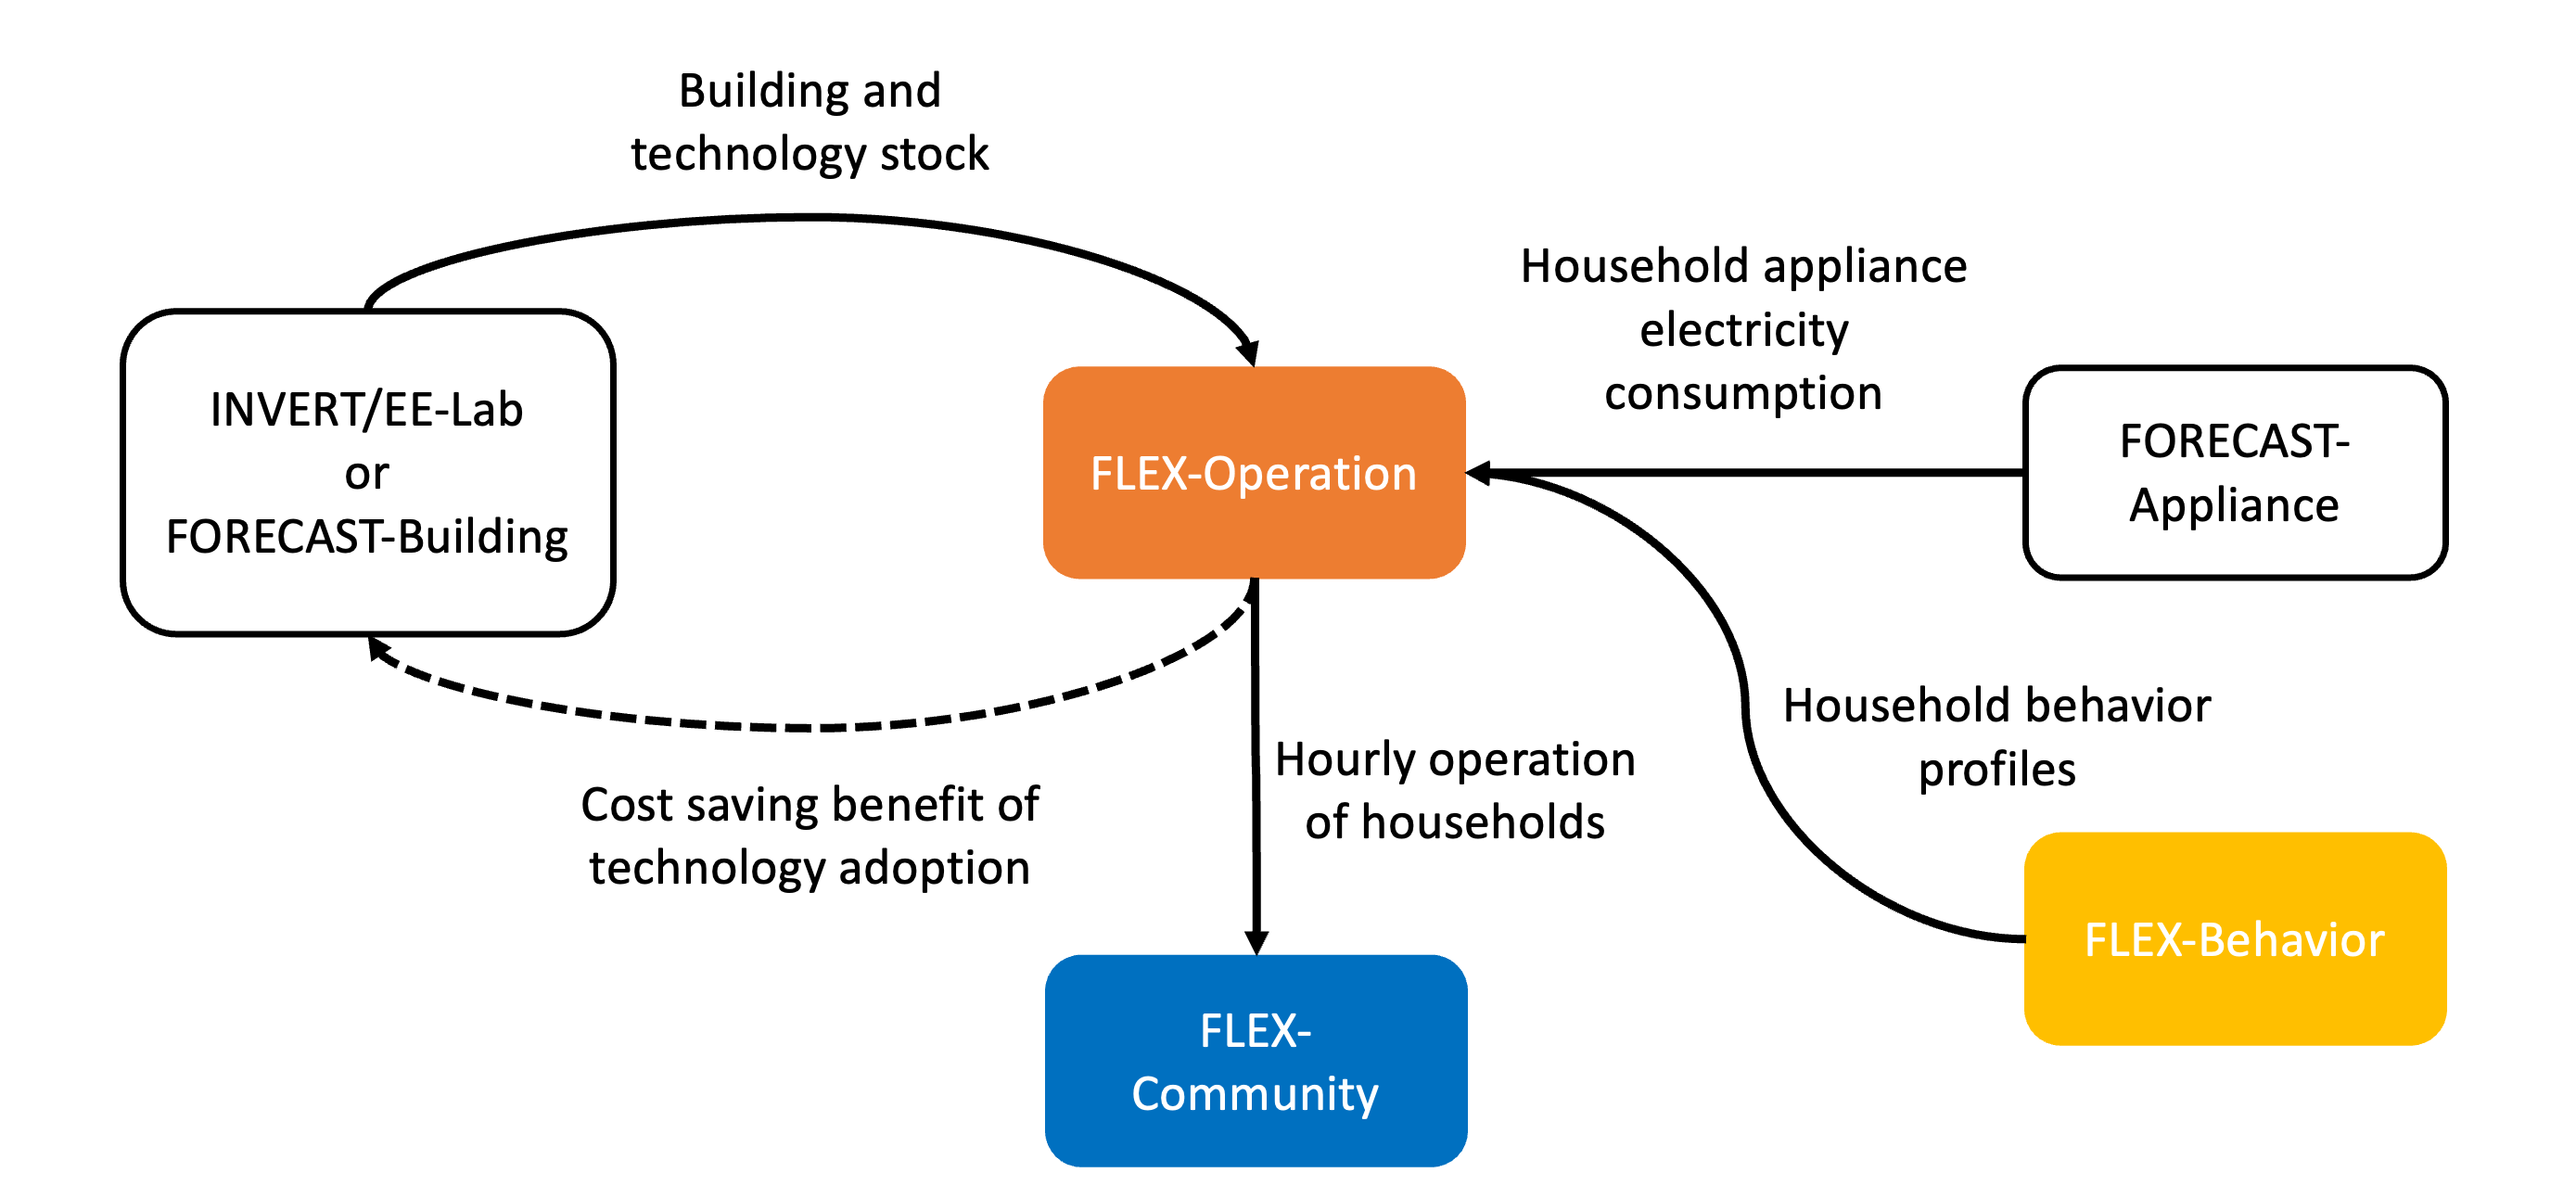
\includegraphics[width=\textwidth]{Images/flex.png}
  \caption{FLEX modeling suite}
  \label{fig:flex}
\end{figure}


%%%%%%%%%%%%%%%%%%%%
\subsubsection{INVERT/EE-Lab and FORECAST-Appliance}


INVERT/EE-Lab and FORECAST-Appliance are the two models that can cover the energy consumption of residential buildings. The two models complement each other and cover the total energy consumption of households. 
However, both INVERT/EE-Lab and FORECAST-Appliance calculate the energy consumption at the annual resolution and cannot model the prosumaging behavior and energy community, which requires an hourly resolution to consider the impact of household behavior, \gls{pv} generation, and energy storage (thermal and battery) on energy consumption. 
In this regard, the FLEX-Operation and FLEX-Community models were developed to improve the building modeling suite and support relevant policy analysis \cite{newtrends}. 


%%%%%%%%%%%%%%%%%%%%
\subsubsection{FLEX-Operation}


FLEX-Operation models the energy system operation of an individual household in hourly resolution.  
It can be used to calculate the energy consumption of each representative building, including operation of technologies (e.g., battery, \gls{pv}, \gls{hp}, etc.) and load profiles in hourly resolution. 
Furthermore, FLEX-Operation can also provide implications for investment decisions, i.e., the energy-saving benefit of technology adoption \cite{newtrends}. 

\begin{figure}[h]
  \centering
  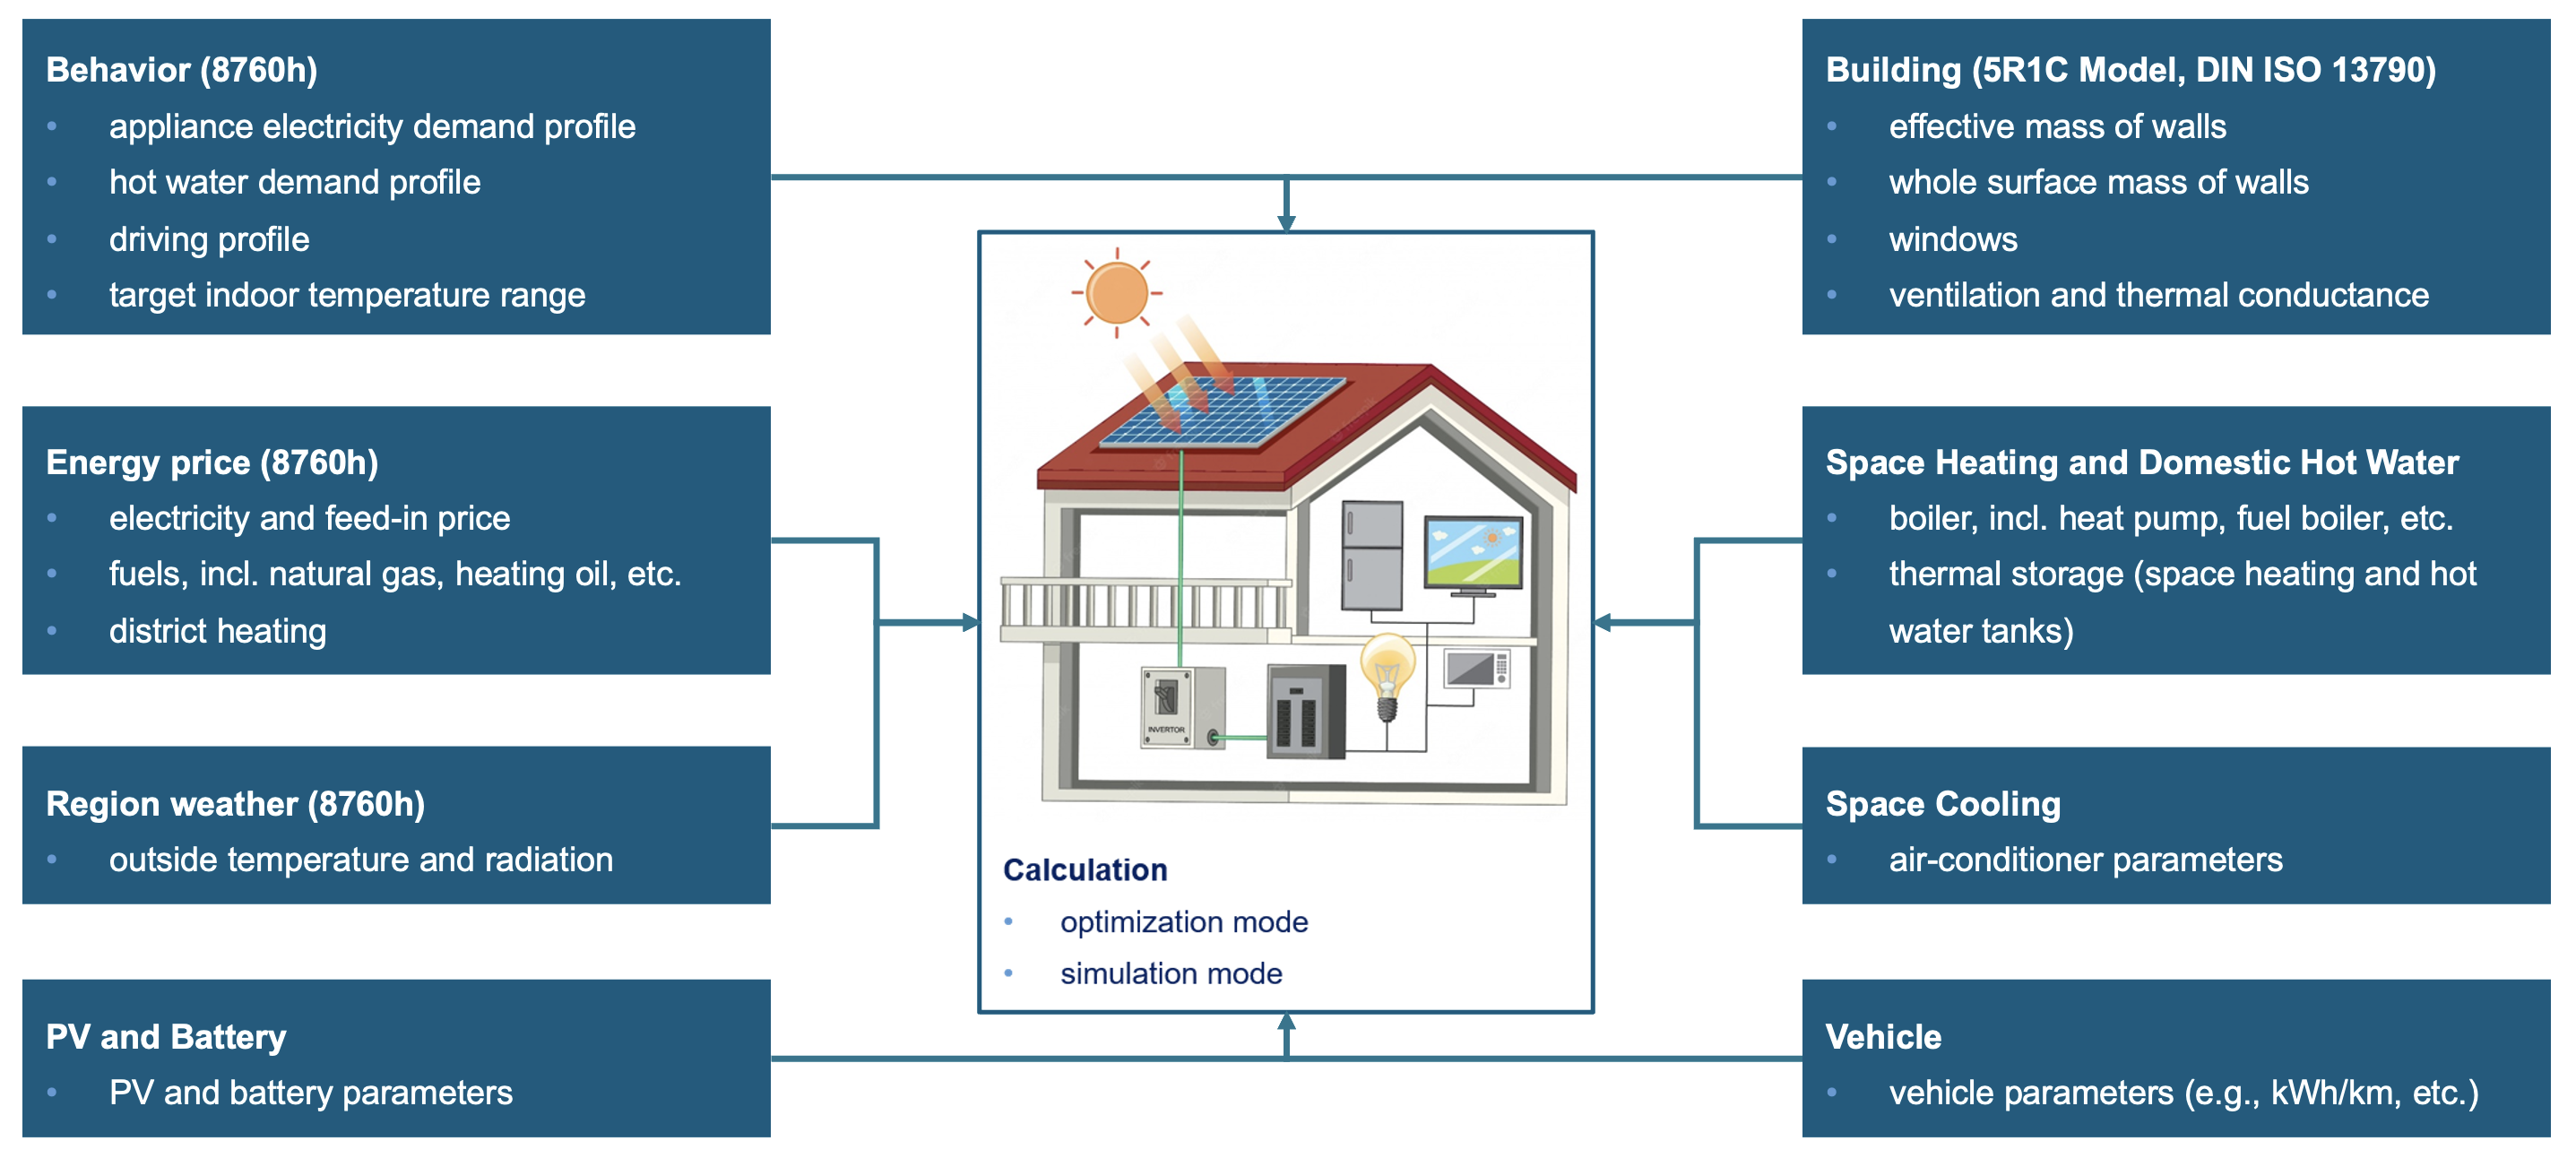
\includegraphics[width=\textwidth]{Images/flex-operation.png}
  \caption{Model structure for individual households}
  \label{fig:flex-operation}
\end{figure}

As shown in figure \ref{fig:flex-operation}, FLEX-Operation considers following five energy services \cite{newtrends}:

\begin{enumerate}
  \item electric appliances, e.g., television, refrigerator, lighting, etc.;
  \item space heating;
  \item domestic hot water;
  \item space cooling;
  \item vehicle. 
\end{enumerate}


%%%%%%%%%%%%%%%%%%%%
\subsubsection{FLEX-Community}


FLEX-Community models the operation of an energy community, i.e., household interaction, aggregator optimisation. 
It can be applied to support the aggregators designing and evaluating business models, as well as making investment decisions, for example, the self-owned battery, \gls{pv} panels, etc. \cite{newtrends}.


%%%%%%%%%%%%%%%%%%%%
\subsubsection{FLEX-Behavior}


FLEX-Behavior models the behavior (activity profile) of households' and corresponding load profiles. 
It generates the hourly activity and energy demand profile of a pre-defined individual household \cite{newtrends}. 
The results include \cite{newtrends}: 

\begin{enumerate}
  \item appliance electricity demand,
  \item domestic hot water demand,
  \item driving profile, and
  \item building occupation.
\end{enumerate}

